\chapter{How the system works, end to end}
\label{ch:system}

\section{One five-second heartbeat}
\begin{simplebox}
The mapper has a heartbeat. Every five seconds it does the same loop, over and over, for as long as it runs:

\begin{enumerate}
\item \textbf{Look.} Ask each machine what containers are running and how busy each one is.
\item \textbf{Listen.} Ask each container who it is currently talking to.
\item \textbf{Update the map.} Add new connections, drop old ones, work out who is the caller on each.
\item \textbf{Judge.} For every service, ask: is this normal for \emph{you}, given how busy the system is?
\item \textbf{Decide.} If something looks wrong, open an incident and work out the likely origin.
\item \textbf{Predict.} Work out which healthy services are likely to be hurt next.
\item \textbf{Show.} Push all of it to the dashboard.
\end{enumerate}

The whole thing takes a few milliseconds of computing. The rest of the five seconds is waiting.
\end{simplebox}

\begin{techbox}
One cycle: (1) collector polls \code{docker ps}, \code{inspect}, \code{stats} and reads \code{/proc/<pid>/net/tcp} and \code{/proc/<pid>/net/dev} per container; (2) \code{GraphStore} merges declared edges (from the Compose file) with observed ones, orients each socket by listening port and expires an observed edge ten minutes after its last sighting; (3) the three engines run in parallel on the same readings (rules score; ML engine with load factor, residual levels, walk, forecast, cascade; fused Hybrid); (4) \code{IncidentManager} builds the evidence for the \emph{active} engine only, calls the root-cause engine and opens, updates or resolves the incident; (5) the server pushes a \code{graph-update} over the WebSocket, coalesced to at most one frame per three seconds. The decision window costs about 0.37\,ms per service on one core.
\end{techbox}

\begin{figure}[H]
\centering
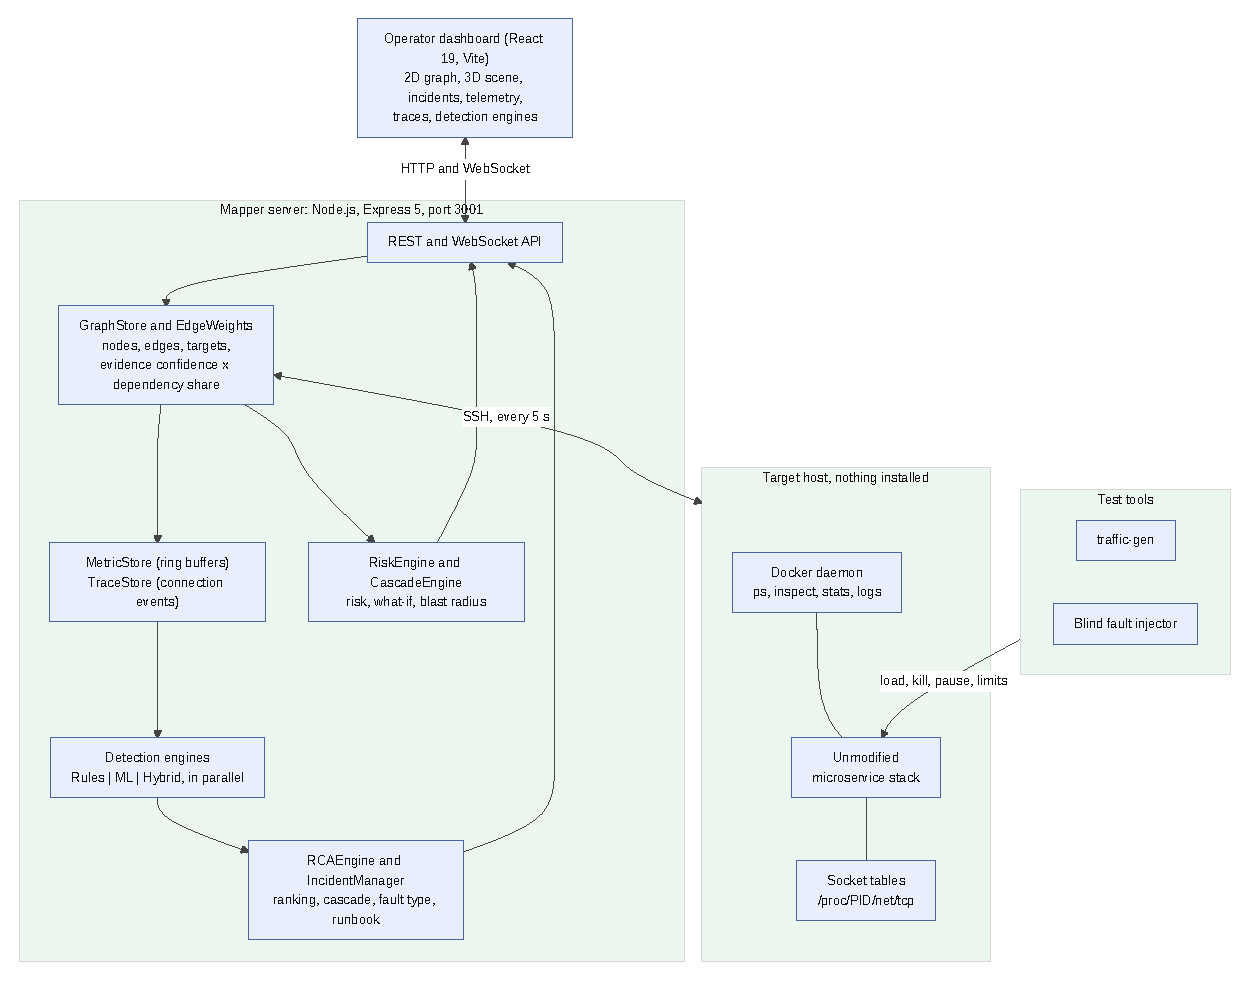
\includegraphics[width=0.98\textwidth,height=0.45\textheight,keepaspectratio]{d_architecture.pdf}
\caption{The architecture. The server reaches the target host over SSH and installs nothing on it. The three engines share the same readings and graph.}
\end{figure}

\section{The five layers, one sentence each}
\begin{center}
\small
\begin{tabularx}{\textwidth}{>{\raggedright\arraybackslash}p{3.1cm}>{\raggedright\arraybackslash}X}
\toprule
\textbf{Layer} & \textbf{What it is}\\
\midrule
Dashboard & A React 19 app. It never polls; the server pushes graph and incident updates over a WebSocket.\\
Server & One Node.js process (Express 5, TypeScript). It owns all state and is the only thing that writes to disk.\\
Connection and collection & One SSH session per target, running commands from a fixed, sanitised catalogue.\\
Target workloads & Unmodified Docker Compose applications. We touch nothing.\\
Test tools & A traffic generator and a blind fault injector, used for experiments only.\\
\bottomrule
\end{tabularx}
\end{center}

\section{The three engines and the switch}
\begin{simplebox}
At the top of the dashboard there is a switch: \textbf{Rules}, \textbf{Hybrid}, \textbf{ML}. These are three different ways of deciding that something is wrong. All three are always running in the background on the same data; the switch only chooses \emph{which one is allowed to open incidents}.

\begin{itemize}
\item \textbf{Rules} is the old-fashioned way: compare each number with the service's own recent history, and complain when it is far off. Fast, easy to explain, but it fires on ordinary noise and often blames the wrong service.
\item \textbf{ML} is our load-aware model plus the random walk. Fewest false alarms, best at naming the true source, but it needs about thirty readings per service before it judges anything.
\item \textbf{Hybrid} (the default) alarms if \emph{either} one alarms, or if a container is stopped, paused or crash-looping. It names the source with the ML ranking.
\end{itemize}
\end{simplebox}

\begin{techbox}
The Hybrid raises the alarm if a container fact holds ($\max_s f_s=1$), or the largest ML level reaches $\tau_\lambda=2$ (twice its own alarm line), or the largest rule score reaches $\tau_\rho=1.25$ (the rules alone must pass $1.25\times$ their own three-sigma line before they are trusted). A container fact raises the alarm at once. In the live system the model and rule conditions must hold for two consecutive windows. The offline evaluation requires two consecutive windows for all three conditions, the stricter reading. Ranking: services with a container fact first, then the ML random-walk order. Keeping all three engines computed on every cycle means that switching engines never starts the learned detector from nothing, and the Detection engines page can show what each decided, computed and predicted at the same moment.
\end{techbox}

\begin{figure}[H]
\centering
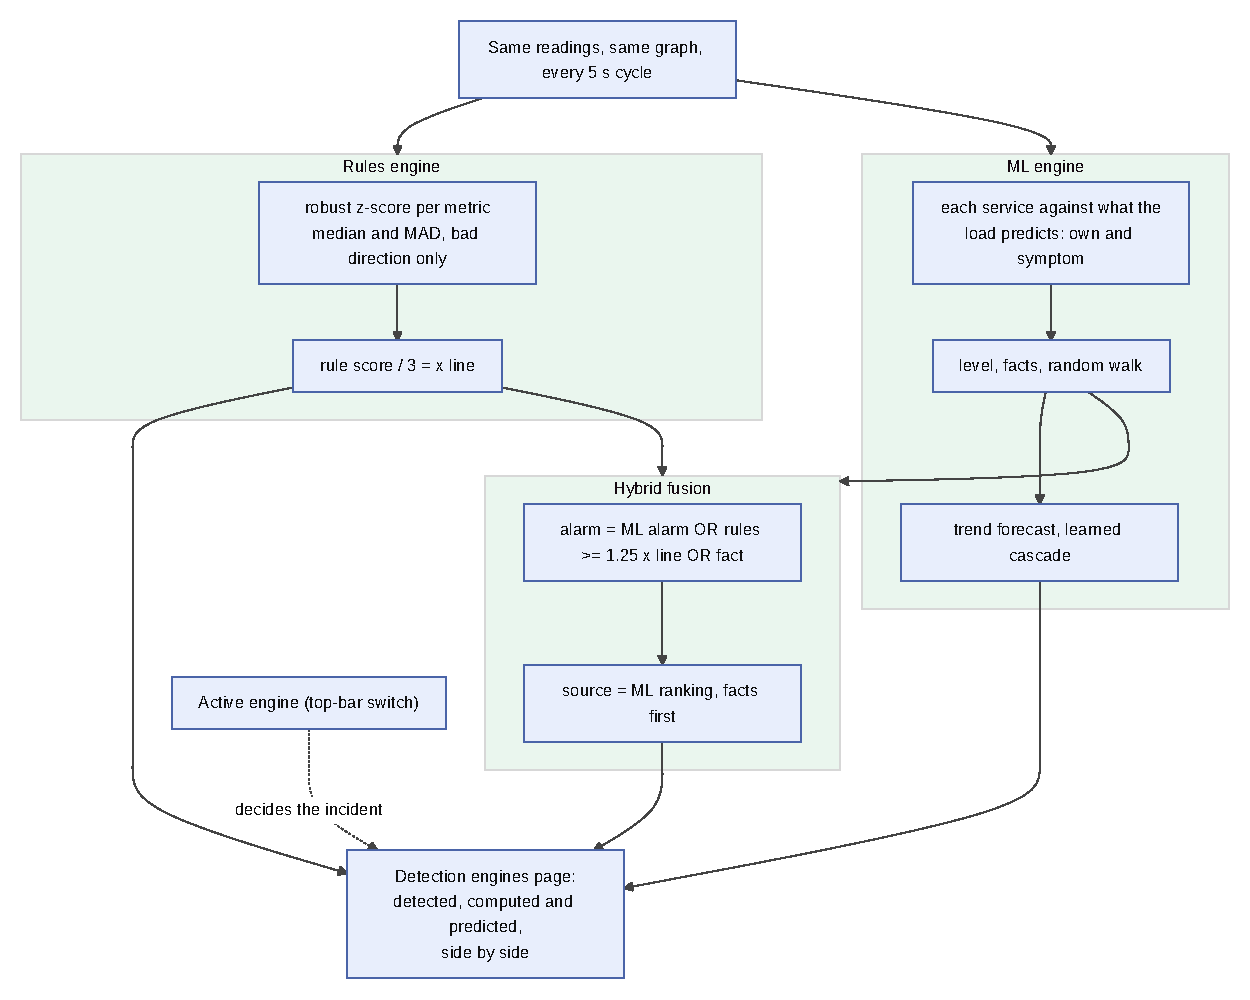
\includegraphics[width=0.98\textwidth,height=0.42\textheight,keepaspectratio]{d_engines_parallel.pdf}
\caption{The three engines run in parallel on the same inputs. The switch chooses which one decides the incident.}
\end{figure}

\begin{saybox}
``All three engines run all the time. The switch does not turn engines on or off; it chooses which one is allowed to open an incident. That is why the Detection engines page can compare them live on the same moment.''
\end{saybox}

\section{Design principles that explain odd-looking code}
Evaluators sometimes ask ``why is it done this strange way?'' The answer is almost always one of these rules.

\begin{enumerate}
\item \textbf{Nothing is installed on the target.} One SSH connection and a fixed set of Docker and \code{/proc} reads. The cost: no per-request data.
\item \textbf{Observed beats declared.} A \code{depends\_on} line is a claim; an open socket is a fact. The graph keeps both but never weighs them equally.
\item \textbf{Unmeasured is missing, never zero.} Zero means ``measured, and it was zero''. A made-up zero looks real on screen.
\item \textbf{Every number can be checked by hand.} Scores are arithmetic over named inputs, and the parts are shown.
\item \textbf{An arrow means ``calls''.} A failure moves \emph{against} the arrow. Reversing it flips everything downstream.
\item \textbf{Compare like with like.} Every model trains on one service's own history; degree, share and criticality are computed inside one project.
\item \textbf{Rules and models stay separate.} Incidents come from the detection engines; the optional Python findings are kept apart so no model is graded on its own output.
\item \textbf{Be light on the target.} Each loop waits for itself, reads each container once per sweep and rediscovers everything every 180 seconds.
\end{enumerate}

\begin{warnbox}
Principle 3 is the one people trip over. In the UI an unmeasured value shows as a dash, not as ``0\%''. If an evaluator sees a dash and asks why, this is the reason.
\end{warnbox}

\section{What happens when a host is slow or down}
\begin{simplebox}
Some machines are so busy that even the simple question ``what containers are running?'' takes a long time. On one overloaded two-gigabyte machine with eighteen heavy services, that question took 45 seconds. If we gave up after 10 seconds the whole machine would disappear from the map, which would look like a mapper bug. So we wait longer, and we built two small tools to tell the two cases apart: one checks the host step by step, the other prints what the mapper believes about it.
\end{simplebox}

\begin{techbox}
Timeouts are sized for a loaded host. \code{npm run check-host} walks one instance and stops at the first failure: port 22, key permissions, login, memory/load/disk, whether \code{docker} answers within 25 s, whether the application answers, which peers each front end calls, whether the mapper is up. \code{npm run mapper-edges} prints the target's status and last-seen time, its nodes and every edge with its evidence and last-seen time. Operational finding (Chapter~6 of the report): a host too small for its workload looks exactly like a mapper fault.
\end{techbox}
